\documentclass{beamer}

% ---- Packages ----

\usepackage[utf8]{inputenc}
\usepackage[british]{babel}
\usepackage{epsfig}
\usepackage{graphics}
\usepackage{tabularx}
\usepackage{amssymb}
\usepackage{amsmath}
\usepackage{xcolor}

% ---- Configuration ----

\usetheme{Madrid}
\useinnertheme{circles}

\definecolor{UDCpink}{RGB}{177,0,114}
\definecolor{UDCgray}{RGB}{100,100,100}

\setbeamercolor{palette primary}{bg=UDCpink,fg=white}
\setbeamercolor{palette secondary}{bg=UDCpink,fg=white}
\setbeamercolor{palette tertiary}{bg=UDCpink,fg=white}
\setbeamercolor{palette quaternary}{bg=UDCpink,fg=white}
\setbeamercolor{structure}{fg=UDCpink} % itemize, enumerate, etc
\setbeamercolor{section in toc}{fg=UDCpink} % TOC sections

% Override palette coloring with secondary
\setbeamercolor{subsection in head/foot}{bg=UDCgray,fg=white}

% ---- Document ----

\title[CLPSM - Workshop 2018]{Scenario Generation for a 2D Videogame using Logic Programming}
\date{A Coruña, \today}
\author[Rafael Alcalde Azpiazu]{Rafael Alcalde Azpiazu \newline \newline Adviser: Pedro Cabalar Fernández}
\institute[UDC]{
\includegraphics[height=2em]{images/logo.png} \newline \textcolor{UDCgray}{FACULTADE DE INFORMÁTICA \\ \textit{Department of Computer Science}} \newline \newline Final degree project}

\begin{document}
	
	\begin{frame}
		\titlepage
	\end{frame}

	\begin{frame}
		\frametitle{Table of Contents}
		\tableofcontents
	\end{frame}

	\AtBeginSection[]
	{
	\begin{frame}
		\frametitle{Table of Contents}
		\tableofcontents[currentsection]
	\end{frame}
	}

	\section{Motivation}
	\subsection{Freeciv}
\begin{frame}
	\frametitle{Freeciv}

	\begin{columns}
		\column{0.75\textwidth}
		
		\begin{itemize}
			\item<1-> Turn-based strategy videogame.
			\item<2-> Created by students of Aarhus University.
			\item<3-> Nowadays developed by an open source community.
		\end{itemize}
		
		\column{0.25\textwidth}
		\centering
		
\includegraphics[width=0.8\textwidth]{images/freeciv.png}
	\end{columns}
\end{frame}

\subsection{Game design}
\begin{frame}
	\frametitle{Game design}
	\begin{itemize}
		\item<1-> Player controls a group of settlers in 4000 B.C.
		\item<2-> 5 ways to end the game:
		\begin{itemize}
			\item<3-> Domination victory.
			\item<3-> Science victory.
			\item<3-> Religion victory.
			\item<3-> Culture victory.
			\item<3-> Score victory.
		\end{itemize}
	\end{itemize}
\end{frame}

\subsection{Types of terrains}
\begin{frame}
\frametitle{Freeciv terrains}
	\begin{columns}
		\column{0.20\textwidth}
		\centering 
\includegraphics[width=0.7\textwidth]{images/grassland.png}
		
		\column{0.80\textwidth}
		\begin{itemize}
			\item Grassland: Common. Units can move easily.
		\end{itemize}
	\end{columns}

	\vspace{1em}
	
	\begin{columns}
		\column{0.20\textwidth}
		\centering 
\includegraphics[width=0.7\textwidth]{images/plains.png}
		
		\column{0.80\textwidth}
		\begin{itemize}
			\item Plains: You can create roads on these cells.
		\end{itemize}
	\end{columns}

	\vspace{1em}
	
	\begin{columns}
		\column{0.20\textwidth}
		\centering 
\includegraphics[width=0.7\textwidth]{images/hills.png}
		
		\column{0.80\textwidth}
		\begin{itemize}
			\item Hills: Units move slowly. +200\% defense bonus.
		\end{itemize}
	\end{columns}

	\vspace{1em}
	
	\begin{columns}
		\column{0.20\textwidth}
		\centering 
\includegraphics[width=0.7\textwidth]{images/forest.png}
		
		\column{0.80\textwidth}
		\begin{itemize}
			\item Forest: +1 production unit. +150\% defense bonus.
		\end{itemize}
	\end{columns}
\end{frame}

\begin{frame}
\frametitle{Freeciv terrains}
	\begin{columns}
		\column{0.20\textwidth}
		\centering 
\includegraphics[width=0.7\textwidth]{images/jungle.png}
		
		\column{0.80\textwidth}
		\begin{itemize}
			\item Jungle: +4 production units with gems/fruit bonus.
		\end{itemize}
	\end{columns}
	
	\vspace{1em}
	
	\begin{columns}
		\column{0.20\textwidth}
		\centering 
\includegraphics[width=0.7\textwidth]{images/mountains.png}
		
		\column{0.80\textwidth}
		\begin{itemize}
			\item Mountains: +300\% defense bonus.
		\end{itemize}
	\end{columns}
	
	\vspace{1em}
	
	\begin{columns}
		\column{0.20\textwidth}
		\centering 
\includegraphics[width=0.7\textwidth]{images/desert.png}
		
		\column{0.80\textwidth}
		\begin{itemize}
			\item Desert: +3 production units with oasis bonus.
		\end{itemize}
	\end{columns}
	
	\vspace{1em}
	
	\begin{columns}
		\column{0.20\textwidth}
		\centering 
\includegraphics[width=0.7\textwidth]{images/swamp.png}
		
		\column{0.80\textwidth}
		\begin{itemize}
			\item Swamp: Fast irrigating. +5/9 production units with peat and spice bonus.
		\end{itemize}
	\end{columns}
\end{frame}

\begin{frame}
\frametitle{Freeciv terrains}
	\begin{columns}
		\column{0.20\textwidth}
		\centering 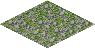
\includegraphics[width=0.7\textwidth]{images/tundra.png}
		
		\column{0.80\textwidth}
		\begin{itemize}
			\item Tundra: Only create roads.
		\end{itemize}
	\end{columns}
	
	\vspace{1em}
	
	\begin{columns}
		\column{0.20\textwidth}
		\centering 
\includegraphics[width=0.7\textwidth]{images/glacier.png}
		
		\column{0.80\textwidth}
		\begin{itemize}
			\item Glacier: No units can pass through.
		\end{itemize}
	\end{columns}
	
	\vspace{1em}
	
	\begin{columns}
		\column{0.20\textwidth}
		\centering 
\includegraphics[width=0.7\textwidth]{images/sea.png}
		
		\column{0.80\textwidth}
		\begin{itemize}
			\item Sea: All types of boats can pass through.
		\end{itemize}
	\end{columns}
	
	\vspace{1em}
	
	\begin{columns}
		\column{0.20\textwidth}
		\centering 
\includegraphics[width=0.7\textwidth]{images/ocean.png}
		
		\column{0.80\textwidth}
		\begin{itemize}
			\item Ocean: Only big ships can pass through.
		\end{itemize}
	\end{columns}
\end{frame}
	
	\section{Project}
	\subsection{First approach}
\begin{frame}
\frametitle{First approach}

\begin{columns}
	\column{0.25\textwidth}
	\centering 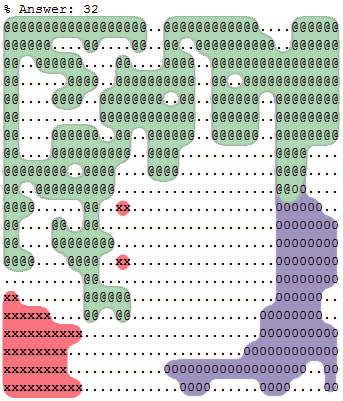
\includegraphics[width=0.7\textwidth]{images/adam.png}
	
	\column{0.75\textwidth}
	\begin{itemize}
		\item<1-> \textit{Answer Set Programming for Procedural Content Generation: A Design Space Approach} \textcolor{UDCpink}{[Smith \& Mateas 11]}
		\item<2-> This approximation creates a single solid island.
		\item<3-> But I need more that one island.
	\end{itemize} 
\end{columns}
	
\end{frame}

\begin{frame}
\frametitle{First approach}

\begin{itemize}
	\item<1-> I created a starting point for generate an island.
	\item<2-> I expanded this points with adjacency rules.
	\item<3-> I added the restriction rules to the adjacent islands not stick together.
	\item<4-> \textcolor{UDCpink}{Problem:} This approach was inefficient with large maps.
\end{itemize}

\end{frame}

\subsection{Second approach}

\begin{frame}
\frametitle{Second approach}

\begin{itemize}
	\item<1-> I divided the map in regions.
	\item<2-> One region is a single island.
	\item<3-> I used the Lua build-in module clingo to call only one region generation.
	\item<4-> Once this work, I generated all the regions with build-in module.
	\item<5-> Finally I added the restriction rules to the regions not stick together.
\end{itemize}

\end{frame}

\subsection{Related work}

\begin{frame}
\frametitle{Related work}

\begin{itemize}
	\item<1-> Add user restrictions to the generation.
	\item<2-> Add all types of terrain.
	\item<3-> Generate player starting points.
	\item<4-> Add a exporter to Freeciv.
\end{itemize}

\end{frame}

	\begin{frame}
		\titlepage
	\end{frame}

\end{document}